\section{Unix fact extraction mechanism in detail}

In this section we want to explain the unix fact extraction mechanism in more detail. Especially we want to explain how we implemented callmon, the executable patching mechanism and metacreator.

\subsection{Overview}

First of all we want to give a quick overview about the whole workflow of the fact extraction tool chain. For more detailed information about the process have a look at section \ref{sec:Tutorial}.

\begin{enumerate}
	\item Building the application with special compiler flags and linking the callmon.{dll,dylib,so}.
	\item Patching the executable results in an executable with just NOPs and a patch file (patch clean).
	\item Patching the executable with the help of an include/exclude file so that we just have specific logging enabled (patch).
	\item Executing the application.
	\item Start logging with the cga toolbar.
	\item Stop logging with the cga toolbar results in cmlog, pre/post modinfo files
	\item The metacreator takes the cmlog and modinfo files and creates a .callmon file
	\item Import and visualize the trace with CGA.
\end{enumerate}

\todo{intro for the class diagram}

\begin{figure}[ht]
\centering
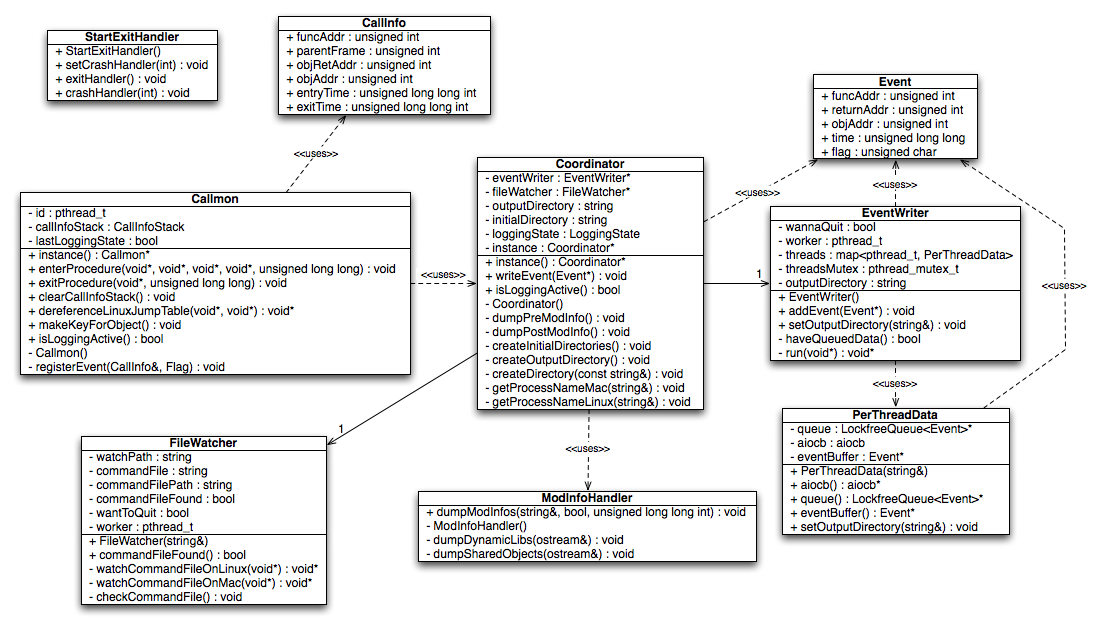
\includegraphics[width=18cm]{images/callmon_class_diagram.png}
\caption{Class diagram of the tracing mechanism}
\end{figure}

\todo{überleitung zu den nächsten sections}

\subsection{Callmon}

\begin{figure}[ht]
\centering
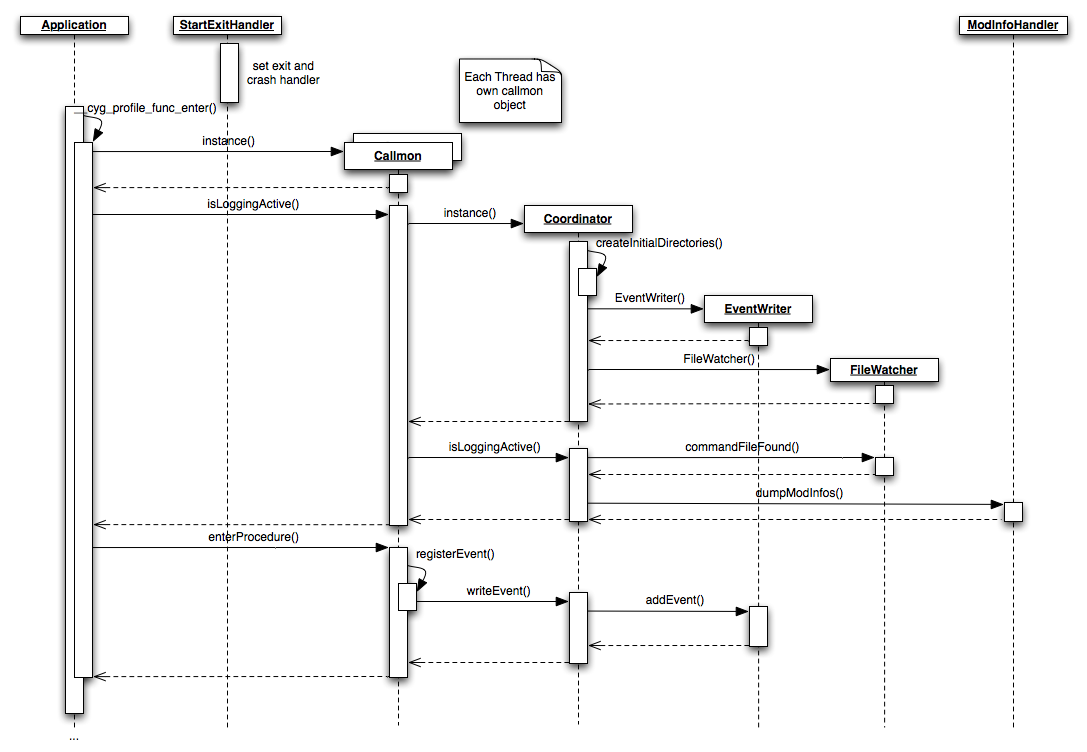
\includegraphics[width=18cm]{images/callmon_sequence_diagram.png}
\caption{Sequence diagram of the function enter procedure}
\end{figure}

Start exit handler: atexit (dtor) + crash (signals)

\begin{verbatim}
__cyg_profile_func_enter, enter procedure, __cyg_profile_func_exit, 
exit procedure, dereferenceLinuxJumpTable
\end{verbatim}

callinfostack, shadowstack

thread local storage
Callmon singleton pro thread (lazy initialization, is the tactic of delaying the creation of an object, the calculation of a value, or some other expensive process until the first time it is needed.)

Event explain structure:
function address, return address, object address, time, flag (entry or exit)

\subsubsection{Coordinator}

singleton

\todo{sequence diagram}

Coordinator - create initial directories (get proc names, linux and mac), modinfohandler, isLoggingActive, output directory

\subsubsection{Filesystem events}

linux filesystem watching

mac file system watching

cga toolbar

\subsubsection{Lockfree event to disk} 

\subsubsection{Asynchronous IO}

\subsection{Patch and Patchclean} 

\subsubsection{ELF patching} 

\subsubsection{MachO patching}

\subsection{Metacreator} 

\subsubsection{Line number caching} 
